\documentclass[12pt]{standalone}
\usepackage{tikz}
\usepackage[T1]{fontenc}
\usepackage{listings}
\lstset{basicstyle=\ttfamily}

\renewcommand{\familydefault}{\sfdefault}
\usetikzlibrary{calc,patterns,decorations.pathreplacing,calligraphy}
\tikzstyle{bag} = [align=center]
\begin{document}
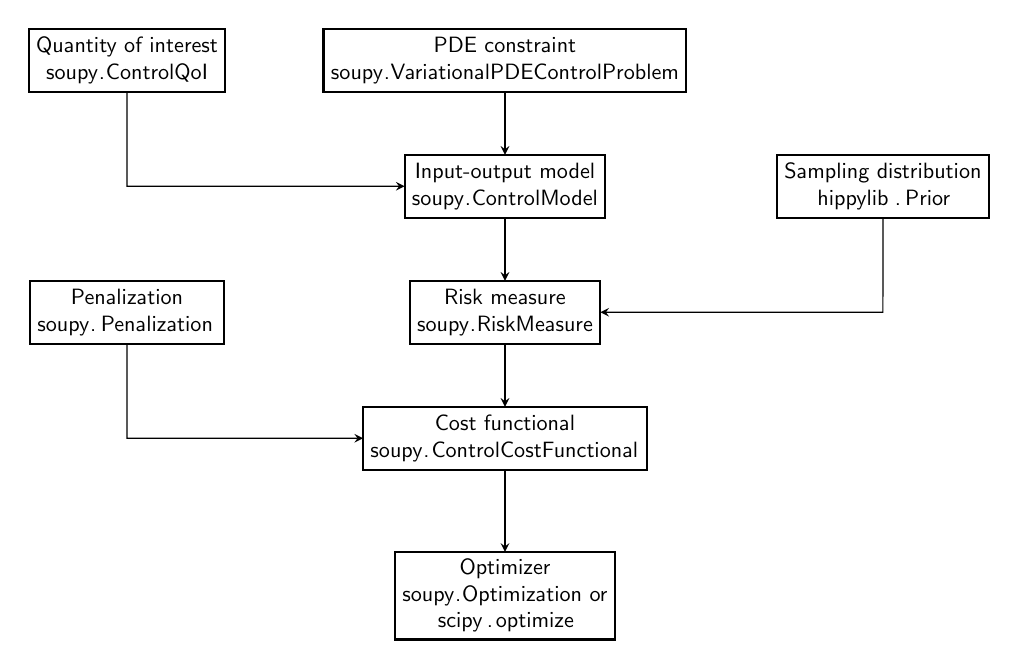
\begin{tikzpicture}[scale = 0.8, transform shape, every node/.style={draw,outer sep=0pt,thick}]    
    
\node[bag] (pde) at (6,0) [minimum width=3cm,minimum height=1cm] {PDE constraint \\ \lstinline{soupy.VariationalPDEControlProblem}};
\node[bag] (qoi) at (0,0) [minimum width=3cm,minimum height=1cm] {Quantity of interest \\ \lstinline{soupy.ControlQoI}};
\node[bag] (model) at (6,-2) [minimum width=3cm,minimum height=1cm] {Input-output model \\ \lstinline{soupy.ControlModel}};
\node[bag] (prior) at (12,-2) [minimum width=3cm,minimum height=1cm] {Sampling distribution \\ \lstinline{hippylib.Prior}};
\node[bag] (risk) at (6,-4) [minimum width=3cm,minimum height=1cm] {Risk measure \\ \lstinline{soupy.RiskMeasure}};
\node[bag] (penalty) at (0,-4) [minimum width=3cm,minimum height=1cm] {Penalization \\ \lstinline{soupy.Penalization}};
\node[bag] (cost) at (6,-6) [minimum width=3cm,minimum height=1cm] {Cost functional \\ \lstinline{soupy.ControlCostFunctional}};

\node[bag] (optimize) at (6,-8.5) [minimum width=3cm,minimum height=1cm] {Optimizer\\ \lstinline{soupy.Optimization} or \\ \lstinline{scipy.optimize}};

\draw[-stealth] (pde.south) -- (model.north); 
\draw[-stealth] (model.south) -- (risk.north); 
\draw[-stealth] (risk.south) -- (cost.north); 
\draw[-stealth] (cost.south) -- (optimize.north); 

\draw[-stealth] (qoi.south) -- (0,-2) -- (model.west); 
\draw[-stealth] (prior.south) -- (12,-4) -- (risk.east); 
\draw[-stealth] (penalty.south) -- (0,-6) -- (cost.west); 


\end{tikzpicture}
\end{document}